\documentclass[11pt]{article}
\title{CS 5114: Theory of Algorithms}
\nonstopmode
%\usepackage[utf-8]{inputenc}
\usepackage{graphicx} % Required for including pictures
\usepackage[figurename=Figure]{caption}
\usepackage{float}    % For tables and other floats
\usepackage{verbatim} % For comments and other
\usepackage{amsmath}  % For math
\usepackage{amssymb}  % For more math
\usepackage{amsthm}  % For theorems and proofs
\usepackage{mathtools}
\usepackage{fullpage} % Set margins and place page numbers at bottom center
\usepackage{paralist} % paragraph spacing
\usepackage{listings} % For source code
\usepackage{subfig}   % For subfigures
\usepackage{sectsty}
\usepackage[super]{nth}
%\usepackage{physics}  % for simplified dv, and
\usepackage{enumitem} % useful for itemization
\usepackage{siunitx}  % standardization of si units
\usepackage{breqn}
\usepackage{chngcntr}
\usepackage{setspace}
\usepackage{multicol}
\usepackage{bookmark}
\usepackage{listings}
\usepackage{color}
\usepackage{hyperref}
\usepackage{titlesec}
\usepackage[linesnumbered, ruled, vlined, commentsnumbered]{algorithm2e}

\setlength{\parskip}{0pt}
\raggedcolumns


\titleformat*{\section}{\normalsize\bfseries}
\titleformat*{\subsection}{\normalsize\bfseries}
\titleformat*{\subsubsection}{\normalsize\bfseries}
\titleformat*{\paragraph}{\normalsize\bfseries}


\begin{document}
\bibliographystyle{plain}

\begin{center}
	\hrule
	\vspace{.4cm}
	{\textbf { \large Optimal Path Finding using Dijkstra's Algorithm with Dynamic Programming}}
\end{center}
\textbf{Name:}\ Matthew Trang \hspace{\fill} \textbf{Date:} \today \\
{ \textbf{Student PID:}} \ mattluutrang \hspace{\fill} \textbf{Project: } 1
\vspace{.4cm}
\hrule

\section*{Abstract}
Finding optimal paths through a two-dimensional (2D) maze is a common problem which can be represented as a graph.
Using Dijkstra's Algorithm, we can find an optimal solution for the shortest path though the maze.
In this paper, a dynamic programming approach is applied to Dijkstra's Algorithm, in both top-down
and bottom-up approaches. The performance of both are compared with respect to accuracy and
efficiency, and contrasted with a recursive approach.

\begin{multicols}{2}
	\section{Introduction}
	In this project, I address the topic of finding the optimal path through a 2D Maze using Dijkstra's Algorithm and
	Dynamic Programming. Dijkstra's Algorithm is a graph-based algorithm that finds the shortest path
	through a series of connected nodes with various weighted, directed edges. The optimal solution of the problem is the
	path which has the lowest cumulative distance between the start and end points.
	For solving 2D mazes, the algorithm can be used to apply a grid of nodes to the maze, and assign
	weights to each node, based on if they are traversable or not \cite{reynolds_python_2020}.

	\subsection{Motivation}
	2-D mazes are common and the task of finding the optimal path through them is a hard problem with many different
	solutions. There are a number of navigation tasks which maze exploration can be used to solve, such
	as city navigation, subway planning, mapping tasks, and others. Finding an optimal minimal path
	solution would improve the functionality of all of these tasks.

	\subsection{Formulation}
	Let ${G}$ be a weighted, directed graph consisting of ${V}$ vertices and ${E}$ edges, such that
	${G=(V,E)}$, where all edge weights are positive and non-zero, or ${w(u, v) \geq 0}$ for all
	edges ${u, v} \in E$. Dijkstra's algorithm maintains a set of vertices ${S}$ which represent
	the set of vertices whose final shortest-path distance has already been determined. The algorithm
	then repeatedly selects the vertex ${u \in V - S}$ with the smallest final shortest-path
	distance, then relaxes all edges from ${u}$ to update the distances of the vertices reachable
	from ${u}$, then adds the vertex ${u}$ to  ${S}$. The algorithm continues the selection,
	relaxation, and exclusion process until the selected vertex ${d}$ is the desired destination.
	Then, it is proven that the path taken by tracing the vertices back from the vertex ${d}$ is the
	smallest distance \cite{cormen_introduction_2009}.	Thus, the algorithm optimizes the minimal
	distance from the start to the end vertices. In this problem, we consider a 2D maze of size ${n
				\times n}$, where ${n}$ is the length in pixels of a side of the maze, and each pixel
	corresponds to a vertex, thus resulting in a graph of size ${n^2}$. Each pixel is connected with
	an edge to a pixel which it shares a side with, meaning each vertex has at most 4 edges.

	\subsection{Sample Input}
	The input to the algorithm is the image of the map that the algorithm must calculate the optimal path for. The image
	consists of a map made of black walls and white paths, with a green pixel for the start position and a red pixel for the end
	position, as shown in Figure \ref{fig:maze}. The maze images can be any number of rows and columns, with any number of paths to the
	start and end positions, as long as there is at least one valid path. Different sample inputs could
	be created using a maze maker. In this project, 23 mazes were created as sample test inputs.
	\begin{figure}[H]
		\centering
		
\includegraphics[width=0.15\textwidth]{"figures/maze_10x10.png"}
		\caption{Sample 10 by 10 maze input for the algorithm\label{fig:maze}}
	\end{figure}

	\section{Applying Dynamic Programming}
	2D Maze solving, and more generally, graph path solving, is suitable for a Dynamic Programming approach as it can be broken down into
	optimal subproblems of the minimum distance to get to each point in the maze, with each point
	building upon the distance of a different point. Dynamic Programming is already being applied to
	the graph path solving problem through Dijkstra's Algorithm. While Dijkstra's Algorithm is more commonly known as a greedy algorithm, it can also
	be
	considered as
	a Dynamic Programming successive approximation procedure, inspired by the Bellman's Principle of
	Optimality \cite{sniedovich_dijkstras_nodate}.

	\subsection{Structure of an Optimal Solution}
	The algorithm uses the computation of the
	distances for each node during previous iterations and saves that value for each node, instead
	of recomputing the value of nodes at each step. Additionally, when the algorithm moves to a new
	vertex ${u}$ in ${V - S}$, if the vertex ${u}$ shares an edge with a vertex in ${S}$, the
	algorithm can skip the edge calculation for that vertex, as it has already calculated the
	optimal minimum distance from the source to that vertex. Thus, the algorithm exhibits optimal
	substructure, the optimal solution to finding the path to the final node encompasses the optimal
	solution of finding the path to each of the nodes before the final node on the optimal path.
	Dijkstra's Algorithm can be solved using a dynamic programming approach by the following.

	\subsection{Computing an Optimal Solution}
	After performing Dijkstra's Algorithm on the graph, the optimal solution for the minimum path
	problem can be found by the following:
	\begin{algorithm}[H]
		\SetAlgoLined
		\SetStartEndCondition{ }{}{}%
		\SetKwProg{Fn}{def}{\string:}{}
		\SetKwFunction{Range}{range}%%
		\SetKw{KwTo}{in}\SetKwFor{For}{for}{\string:}{}%
		\SetKwIF{If}{ElseIf}{Else}{if}{:}{elif}{else:}{}%
		\SetKwFor{While}{while}{:}{fintq}%
		\AlgoDontDisplayBlockMarkers\SetAlgoNoEnd\SetAlgoNoLine%
		\KwData{${G}$ is a graph, ${d}$ is the destination node, which has been reached}
		\KwResult{shortest path}
		\Begin{
			${path}$  is initialized as an empty vector\\
			\While {$d$.parent exists}{
				${path}$ appended with ${d.parent}$\\
				${d \leftarrow d.parent}$\\
			}
			\Return{${path}$}
		}
		\caption{GetSolution(${G}$, ${d}$)\label{get-soln}}
	\end{algorithm}

	\subsubsection{Naive Recursive Algorithm}
	While Dijkstra's Algorithm is innately a Dynamic Programming approach, it is possible to write a
	much more inefficient purely recursive method to solve the optimal shortest-path problem. This
	method would not use precalculated values, but instead would calculate the distances recursively
	for each node in the set ${S}$. The algorithm for the recursive approach to the maze solving
	problem is as follows:

	\begin{algorithm}[H]
		\SetAlgoLined
		\SetStartEndCondition{ }{}{}%
		\SetKwProg{Fn}{def}{\string:}{}
		\SetKwFunction{Range}{range}%%
		\SetKw{KwTo}{in}\SetKwFor{For}{for}{\string:}{}%
		\SetKwIF{If}{ElseIf}{Else}{if}{:}{elif}{else:}{}%
		\SetKwFor{While}{while}{:}{fintq}%
		\AlgoDontDisplayBlockMarkers\SetAlgoNoEnd\SetAlgoNoLine%
		\KwData{${G=(V,E)}$ is the graph, ${s}$ is the source node, ${d}$ is the destination node, ${p}$
			is the current path}
		\KwResult{shortest path}
		\Begin{
			\If{${s == d}$ }{
				\Return{${p}$}
			}
			${p}$ is appended with ${s}$\\
			${n}$ is initialized as empty \\
			\For {${v \in V[s]}$ }{
				\If{${v \notin p}$ }{
					${np = }$ MazeRecur(${G, v, d, p}$)\\
					\If{${np.length() < n.length()}$ }{
						${n = np}$\\
					}
				}
			}
			\Return{${n}$}
		}
		\caption{MazeRecur(${G}$, ${s}$, ${d}$, ${p}$)\label{recur}}
	\end{algorithm}

	The for loop inside each call is ${\Theta(n^2)}$, where ${n^2}$ is the number of vertices in the
	graph and ${n}$ is the length of one of the sides of the maze, as it must check if the vertex it checks is in the path list, which could be as large as ${n^2}$, and the
	recursion itself is ${\Theta(n^4)}$ as it could potentially have to check for
	every node until it finds the finish node, and this could occur for every node. Thus, for the whole algorithm, the efficiencies are
	${\Theta(n^6)}$, Big-O${(n^6)}$, and
	${\Omega(n^2)}$ in the best case if the maze is linear with no branches.

	\subsubsection{Top-Down Dynamic Programming}
	The Top-Down/Memoized Algorithm for 2D Maze Solving aims to use Dijkstra's Algorithm in a way
	that writes the procedure recursively in a natural way, and then uses the results of the saved
	subproblems if they have previously been computed, or calculates them if they haven't been
	computed.
	The pseudocode for the Top-Down approach to Dijkstra's Algorithm is as follows:

	\begin{algorithm}[H]
		\SetAlgoLined
		\SetStartEndCondition{ }{}{}%
		\SetKwProg{Fn}{def}{\string:}{}
		\SetKwFunction{Range}{range}%%
		\SetKw{KwTo}{in}\SetKwFor{For}{for}{\string:}{}%
		\SetKwIF{If}{ElseIf}{Else}{if}{:}{elif}{else:}{}%
		\SetKwFor{While}{while}{:}{fintq}%
		\AlgoDontDisplayBlockMarkers\SetAlgoNoEnd\SetAlgoNoLine%
		\KwData{${R=V-S}$ is the set of nodes that have yet to be visited}
		\KwResult{the node with the shortest distance from the source}
		\Begin{
			${d = \infty}$ \\
			${n = None}$\\
			\For {${u \in V}$ }{
				\If{${u.dist<d}$}{
					${d = u.dist}$\\
					${n = u}$\\
				}
			}
			\Return{${n}$}
		}
		\caption{GetMinDist(${R}$)\label{min-dist}}
	\end{algorithm}

	\begin{algorithm}[H]
		\SetAlgoLined
		\SetStartEndCondition{ }{}{}%
		\SetKwProg{Fn}{def}{\string:}{}
		\SetKwFunction{Range}{range}%%
		\SetKw{KwTo}{in}\SetKwFor{For}{for}{\string:}{}%
		\SetKwIF{If}{ElseIf}{Else}{if}{:}{elif}{else:}{}%
		\SetKwFor{While}{while}{:}{fintq}%
		\AlgoDontDisplayBlockMarkers\SetAlgoNoEnd\SetAlgoNoLine%
		\KwData{${R}$ is the set of nodes that have yet to be visited, ${u}$ is the node to update
			the neighbors of}
		\Begin{
			\For {${v \in R[u]}$ }{
				\If{${v.dist > u.dist + E[v,u]}$}{
					${v.dist = u.dist + E[v,u]}$\\
					${v.parent = u}$\\
				}
			}
		}
		\caption{UpdateNeighbors(${R}$, ${u}$)\label{update}}
	\end{algorithm}

	\begin{algorithm}[H]
		\SetAlgoLined
		\SetStartEndCondition{ }{}{}%
		\SetKwProg{Fn}{def}{\string:}{}
		\SetKwFunction{Range}{range}%%
		\SetKw{KwTo}{in}\SetKwFor{For}{for}{\string:}{}%
		\SetKwIF{If}{ElseIf}{Else}{if}{:}{elif}{else:}{}%
		\SetKwFor{While}{while}{:}{fintq}%
		\AlgoDontDisplayBlockMarkers\SetAlgoNoEnd\SetAlgoNoLine%
		\KwData{${G=(V,E)}$ is a graph, ${s}$ is the start node, ${d}$ is the destination node}
		\KwResult{shortest path}
		\Begin{
			G = G - s\\
			\If{${s==d}$ }{
				\Return{${[s]}$}
			}
			UpdateNeighbors(${V-S}$, ${u}$)\\
			${u}$ = GetMinDist(${G}$)\\
			\If{${u}$ is ${None}$ }{
				\Return{${None}$}
			}
			${path}$ += DijkRecurTD${(u, d)}$\\
			\Return{${path}$}\\
		}
		\caption{DijkRecurTD(${G}$, ${s}$, ${d}$)\label{tdrc}}
	\end{algorithm}

	\begin{algorithm}[H]
		\SetAlgoLined
		\SetStartEndCondition{ }{}{}%
		\SetKwProg{Fn}{def}{\string:}{}
		\SetKwFunction{Range}{range}%%
		\SetKw{KwTo}{in}\SetKwFor{For}{for}{\string:}{}%
		\SetKwIF{If}{ElseIf}{Else}{if}{:}{elif}{else:}{}%
		\SetKwFor{While}{while}{:}{fintq}%
		\AlgoDontDisplayBlockMarkers\SetAlgoNoEnd\SetAlgoNoLine%
		\KwData{${G=(V,E)}$ is a graph, ${s}$ is the start node, ${d}$ is the destination node}
		\KwResult{shortest path}
		\Begin{
			${S \leftarrow \emptyset}$ \\
			initialize ${u.dist= \infty: \forall u \in V}$\\
			${s.dist = 0}$\\
			DijkRecurTD(G, s, d)\\
			\Return{\text{GetSolution(G, d)}}
		}
		\caption{DijkstraTD(${G}$, ${s}$, ${d}$)\label{td}}
	\end{algorithm}

	The runtime is ${\Theta(|E|*T_{update} + |V|*T_{getmin})}$ as it must run an update for each
	edge, and get the minimum for each vertex. The time to update the edges is constant, as each
	vertex only has 4 edges, and the GetMinDist function is ${\Theta(|V|)}$ as it is must search to find the minimum value
	in the set. Thus, for the whole algorithm, the efficiencies are
	${\Theta(4|V| + |V|^2)}=\Theta(n^4)$, Big-O${(n^4)}$, and
	${\Omega(n^2)}$ in the best case if the maze is simple.

	\subsubsection{Bottom-Up Dynamic Programming}
	The Bottom-Up approach is similar to the Top-Down approach, but instead of recursively updating
	the graph, it would instead update the graph in a bottom-up fashion.

	\begin{algorithm}[H]
		\SetAlgoLined
		\SetStartEndCondition{ }{}{}%
		\SetKwProg{Fn}{def}{\string:}{}
		\SetKwFunction{Range}{range}%%
		\SetKw{KwTo}{in}\SetKwFor{For}{for}{\string:}{}%
		\SetKwIF{If}{ElseIf}{Else}{if}{:}{elif}{else:}{}%
		\SetKwFor{While}{while}{:}{fintq}%
		\AlgoDontDisplayBlockMarkers\SetAlgoNoEnd\SetAlgoNoLine%
		\KwData{${G=(V, E)}$, ${s}$, ${d}$}
		\KwResult{shortest path}
		\Begin{
			${S \leftarrow \emptyset}$ \\
			initialize ${u.dist= \infty: \forall u \in V}$\\
			${s.dist = 0}$\\
			\For {${i=1 \text{ to } V.size}$ }{
				${u}$ = GetMinDist(${V-S}$)\\
				${S \leftarrow S \cup {u}}$\\
				\If{${u==d}$ }{
					break
				}
				UpdateNeighbors(${V-S}$, ${u}$)
			}
			\Return{\text{GetSolution(G, d)}}
		}
		\caption{DijkstraBU(${G}$, ${s}$, ${d}$)\label{bd}}
	\end{algorithm}

	The runtime of the Bottom-Up approach is exactly the same as the Top-Down approach, with
	potentially more time saved due to less function calls, but still the same asymptotic behavior. Thus, the efficiencies are
	$\Theta(n^4)$, Big-O${(n^4)}$, and
	${\Omega(n^2)}$.

	\subsection{Sample Output}
	Figure \ref{fig:output_maze} shows the output of the Dijkstra's Algorithm for the 10 by 10 maze
	in Figure \ref{fig:maze}. The optimal shortest path from the green start pixel to the red finish
	pixel follows the blue path. In this case, the optimal path was a length of 19 pixels, which can
	be verified manually. Each algorithm was able to correctly come to this result, thus all three
	are equally accurate.

	\begin{figure}[H]
		\centering
		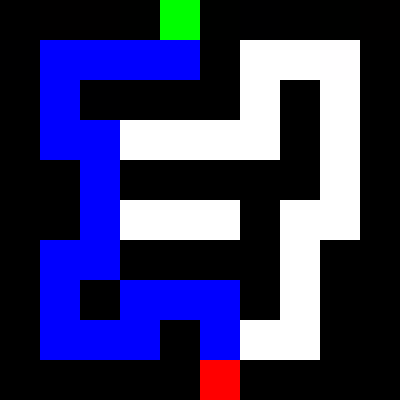
\includegraphics[width=0.2\textwidth]{figures/output_maze_10x10.png}
		\caption{Output of a optimally navigated maze, where the blue line represents the shortest
			path. \label{fig:output_maze}}
	\end{figure}

	Another example of the program output is shown in Figure \ref{fig:maze_big}, which uses a 40 by
	40 pixel maze as input.

	\begin{figure}[H]
		\centering
		\subfloat[\centering
			Input]{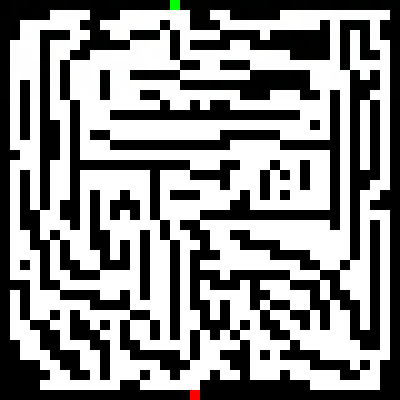
\includegraphics[width=0.2\textwidth]{figures/input_maze_40x40_hard.png}}
		\qquad
		\subfloat[\centering Output]{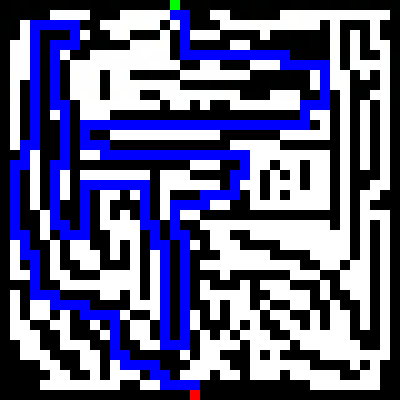
\includegraphics[width=0.2\textwidth]{figures/output_maze_40x40_hard.png}}
		\caption{Input and Output for a 40x40 maze\label{fig:maze_big}}
	\end{figure}

	\section{Benchmarks}
	In all cases, the algorithms were benchmarked using the time library in Python, which allows for
	precise time values in fractional seconds from a performance counter. The timing results do not
	include time spent loading in or annotating the images. It can be seen that the time taken for
	the recursive algorithm is exponentially larger than that for the Dynamic Programming
	approaches, with the 30 by 30 maze taking 3.19 seconds for the recursive approach compared to 0.05
	seconds for both DP approaches. In fact, when moving to the 40 by 40 maze, the recursive
	approach takes over 15 minutes, and is thus not considered in the graph. The runtimes of the two
	DP algorithms are very similar, following expectations.
	\begin{figure}[H]
		\centering
		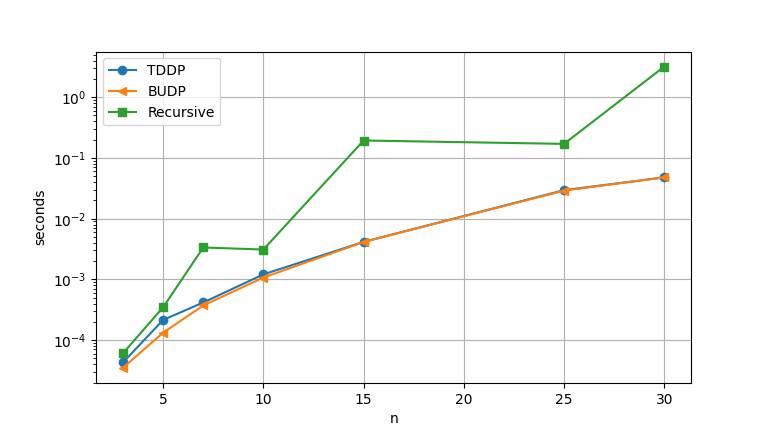
\includegraphics[width=0.4\textwidth]{figures/benchmark_log.png}
		\caption{Runtimes of the 3 different algorithms for different ${n}$ values on a log
			scale.\label{fig:benchmark}}
	\end{figure}

	\section{Parameters and Extensions}
	The program parameters that can affect the running time include the choice of input maze
	dimensions, with the choice of ${n}$ maze length size having a squared effect on the number of
	nodes. This has a large impact on the runtime of the algorithms, as the more nodes, the more
	iterations of distance calculations must be done. The impact is shown in Figure \ref{fig:benchmark}. The difficulty of the maze path is also a factor in the
	algorithm, as the deeper
	the path is from the start to the end node, and the more branching paths which also lead towards
	the destination, the more iterations the algorithm has to perform to compare between the paths. The effect of an easy, medium,
	and hard difficulty maze is shown in Figure \ref{fig:diff}.
	\begin{figure}[H]
		\centering
		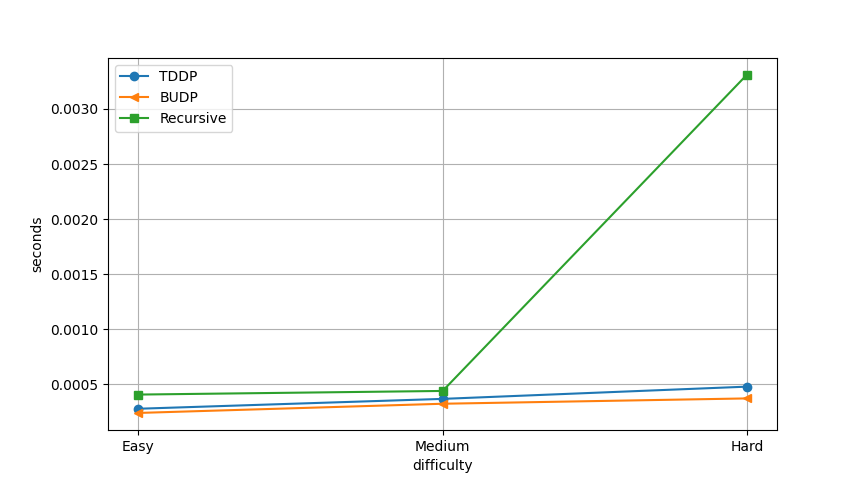
\includegraphics[width=0.4\textwidth]{figures/difficulty_7.png}
		\caption{Runtimes of the three methods on varying levels of difficulties for a 5 by 5 maze. \label{fig:diff}}
	\end{figure}

	However, the accuracy of the path finding algorithm is not affected by the difficulty of the
	maze, as Dijkstra's Algorithm has been proven to be optimal \cite{cormen_introduction_2009}, and
	indeed, the output of the algorithms all follow the same minimal path which has been manually
	verified as optimal.
	% The
	% maze algorithm currently only works with black and white mazes, and could potentially be
	% modified with edge detection code to allow for color variant mazes, which could also introduce
	% room for experimentation with varying edge weights, which was not tested in this implementation. \\
	% An extension of the algorithm could improve on the efficiency of calculation by using a
	% different data structure such as a Fibonacci heap \cite{715934}.

	\section{Conclusion}
	In conclusion, the optimal path through a 2D maze can be solved using Dijkstra's Algorithm with
	Dynamic Programming as an efficient and effective method as an alternative to some other
	heuristic based maze algorithm, or a recursive implementation.

	\bibliography{proj1.bib}

\end{multicols}

\end{document}
